\chapter{Community concept}
\label{CommunityConcept}
I dette kapitel skal konceptet bag TonePrint communitiet forklares med udgangspunkt i at der tilsidst skal tages et valg af hvilken det vi skal hjælpe med at udvikle.\\

\section{Conceptual model}
\label{ConceptualModel}

\begin{figure}[H]
	\centering
	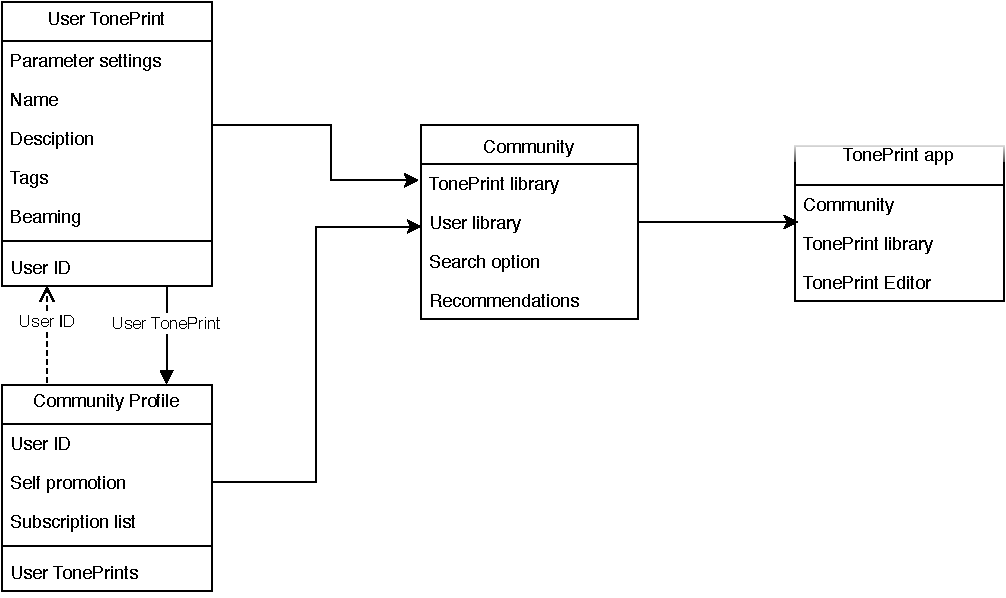
\includegraphics[width=\textwidth]{CommunityFirstDraft.pdf}
	\caption{a graphical overview of the TonePrint Community concept}
	\label{fig:CommunityConceptualModel}
\end{figure}

\subsection{Use case}

\begin{figure}[H]
	\centering
	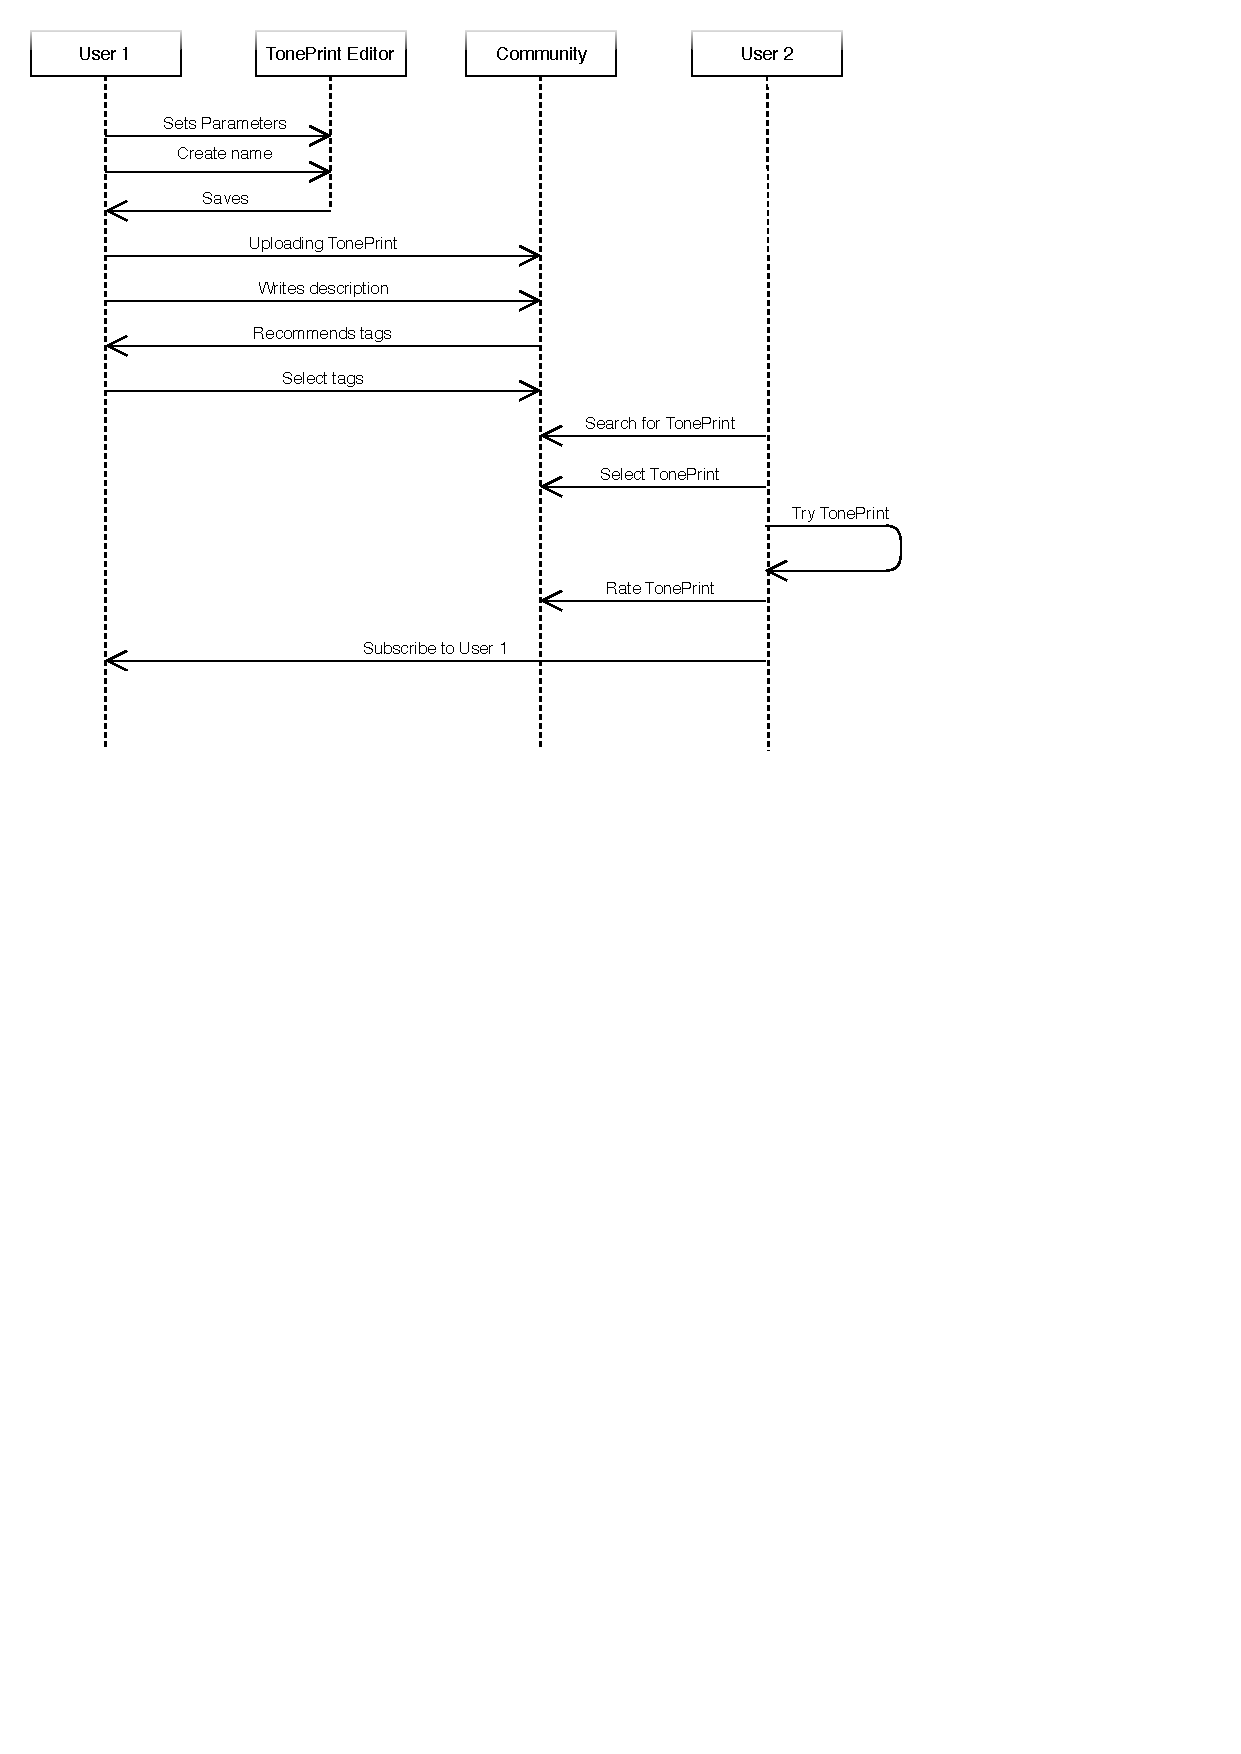
\includegraphics[width=\textwidth]{CommunityUseCaseOne.pdf}
	\caption{a graphical overview of the TonePrint Community use case}
	\label{fig:CommunityConceptualUseCase}
\end{figure}